% Options for packages loaded elsewhere
\PassOptionsToPackage{unicode}{hyperref}
\PassOptionsToPackage{hyphens}{url}
%
\documentclass[
]{book}
\usepackage{amsmath,amssymb}
\usepackage{iftex}
\ifPDFTeX
  \usepackage[T1]{fontenc}
  \usepackage[utf8]{inputenc}
  \usepackage{textcomp} % provide euro and other symbols
\else % if luatex or xetex
  \usepackage{unicode-math} % this also loads fontspec
  \defaultfontfeatures{Scale=MatchLowercase}
  \defaultfontfeatures[\rmfamily]{Ligatures=TeX,Scale=1}
\fi
\usepackage{lmodern}
\ifPDFTeX\else
  % xetex/luatex font selection
\fi
% Use upquote if available, for straight quotes in verbatim environments
\IfFileExists{upquote.sty}{\usepackage{upquote}}{}
\IfFileExists{microtype.sty}{% use microtype if available
  \usepackage[]{microtype}
  \UseMicrotypeSet[protrusion]{basicmath} % disable protrusion for tt fonts
}{}
\makeatletter
\@ifundefined{KOMAClassName}{% if non-KOMA class
  \IfFileExists{parskip.sty}{%
    \usepackage{parskip}
  }{% else
    \setlength{\parindent}{0pt}
    \setlength{\parskip}{6pt plus 2pt minus 1pt}}
}{% if KOMA class
  \KOMAoptions{parskip=half}}
\makeatother
\usepackage{xcolor}
\usepackage{longtable,booktabs,array}
\usepackage{calc} % for calculating minipage widths
% Correct order of tables after \paragraph or \subparagraph
\usepackage{etoolbox}
\makeatletter
\patchcmd\longtable{\par}{\if@noskipsec\mbox{}\fi\par}{}{}
\makeatother
% Allow footnotes in longtable head/foot
\IfFileExists{footnotehyper.sty}{\usepackage{footnotehyper}}{\usepackage{footnote}}
\makesavenoteenv{longtable}
\usepackage{graphicx}
\makeatletter
\def\maxwidth{\ifdim\Gin@nat@width>\linewidth\linewidth\else\Gin@nat@width\fi}
\def\maxheight{\ifdim\Gin@nat@height>\textheight\textheight\else\Gin@nat@height\fi}
\makeatother
% Scale images if necessary, so that they will not overflow the page
% margins by default, and it is still possible to overwrite the defaults
% using explicit options in \includegraphics[width, height, ...]{}
\setkeys{Gin}{width=\maxwidth,height=\maxheight,keepaspectratio}
% Set default figure placement to htbp
\makeatletter
\def\fps@figure{htbp}
\makeatother
\setlength{\emergencystretch}{3em} % prevent overfull lines
\providecommand{\tightlist}{%
  \setlength{\itemsep}{0pt}\setlength{\parskip}{0pt}}
\setcounter{secnumdepth}{5}
\usepackage{booktabs}
\usepackage{amsthm}
\makeatletter
\def\thm@space@setup{%
  \thm@preskip=8pt plus 2pt minus 4pt
  \thm@postskip=\thm@preskip
}
\makeatother
\ifLuaTeX
  \usepackage{selnolig}  % disable illegal ligatures
\fi
\usepackage[]{natbib}
\bibliographystyle{apalike}
\IfFileExists{bookmark.sty}{\usepackage{bookmark}}{\usepackage{hyperref}}
\IfFileExists{xurl.sty}{\usepackage{xurl}}{} % add URL line breaks if available
\urlstyle{same}
\hypersetup{
  pdftitle={En befolkning blander sig},
  pdfauthor={Christian Albrekt Larsen og Hans-Peter Y. Qvist (Red.); Med bidrag fra Jeppe Fjeldgaard Larsen, Laciné E. Diop,\ldots{} Anders? Anna?},
  hidelinks,
  pdfcreator={LaTeX via pandoc}}

\title{En befolkning blander sig}
\author{Christian Albrekt Larsen og Hans-Peter Y. Qvist (Red.) \and Med bidrag fra Jeppe Fjeldgaard Larsen, Laciné E. Diop,\ldots{} Anders? Anna?}
\date{2024-04-19}

\begin{document}
\maketitle

{
\setcounter{tocdepth}{1}
\tableofcontents
}
\hypertarget{forord}{%
\chapter*{Forord}\label{forord}}
\addcontentsline{toc}{chapter}{Forord}

Måske et forord her.

Samt en smart \emph{måde} at præsenterer \textbf{indholdsfortegnelse} og \textbf{\emph{overblik}} i dette format. Evt. korte summaries/abstracts til de enkelte kapitler?

Vi kan linke til andre \protect\hyperlink{kap1}{kapitler} og refencer i henhold til bibtex standarder \citep{xie2015}.

\hypertarget{kap1}{%
\chapter{En befolkning blander sig}\label{kap1}}

\begin{figure}
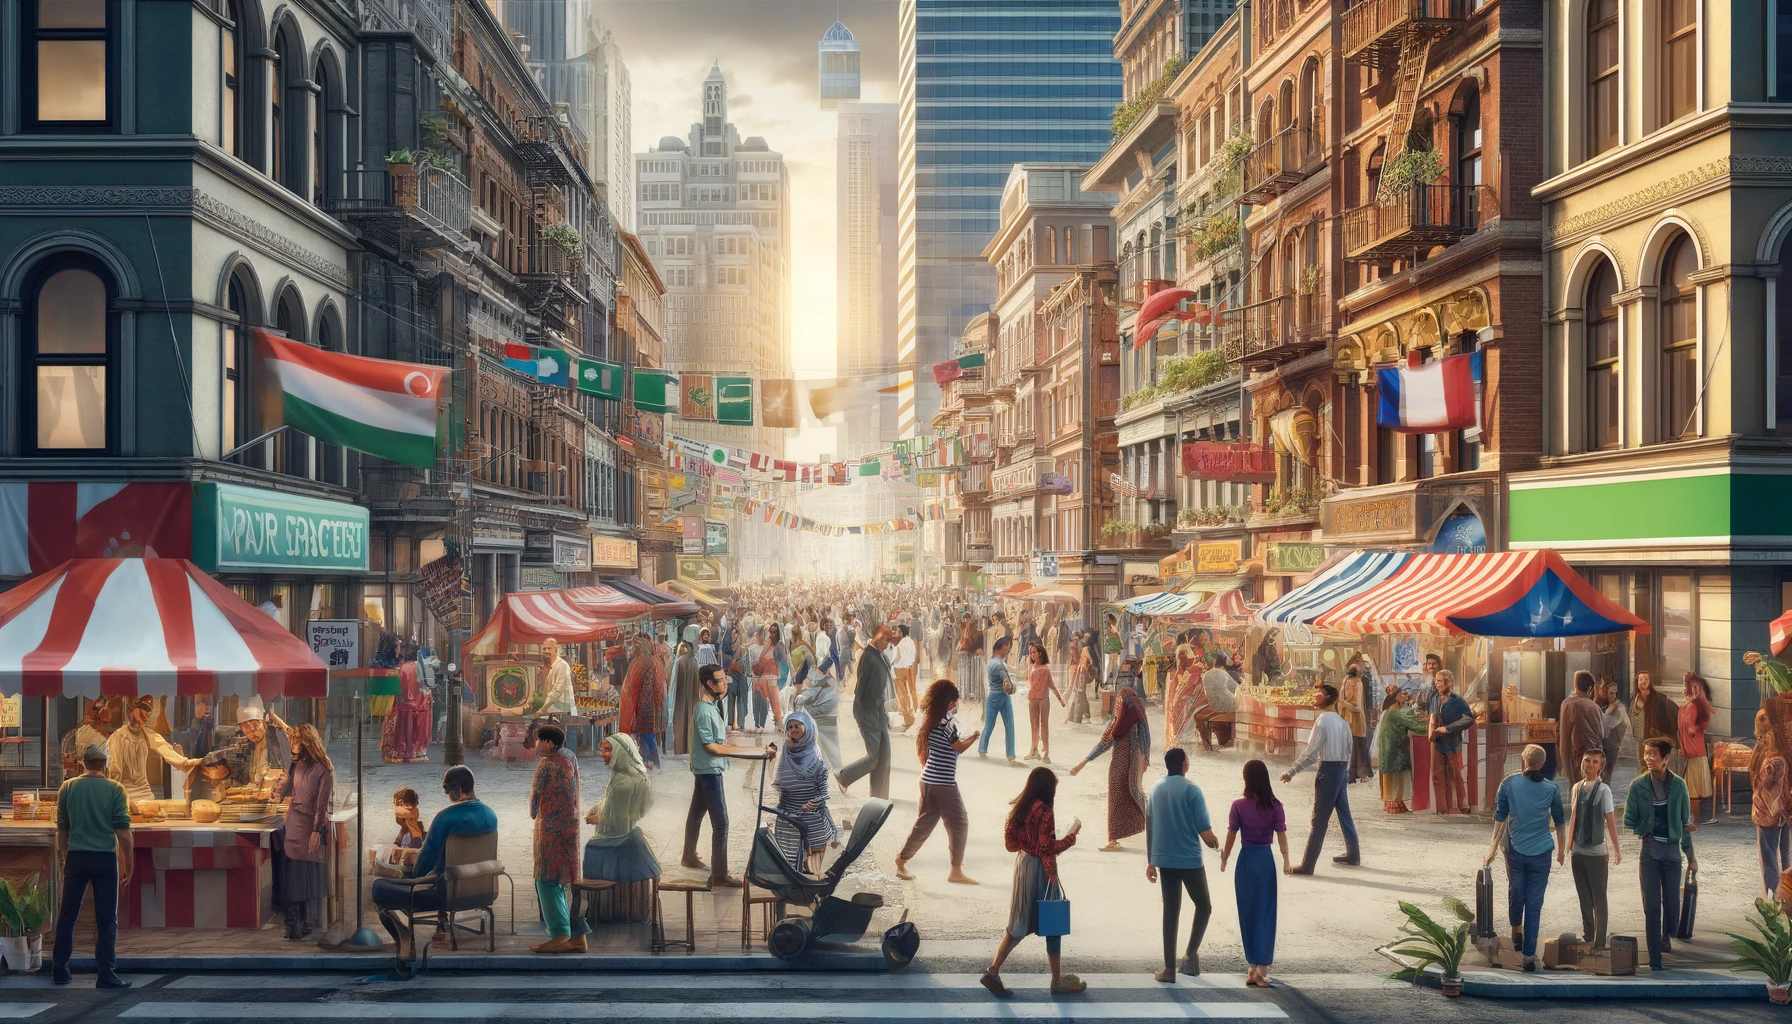
\includegraphics[width=24.89in]{images/dalle-smeltedige} \caption{Smeltedigen, tolket af en AI model}\label{fig:fig-smelte}
\end{figure}

test \citep{xie2015}.

\hypertarget{kap2}{%
\chapter{Partnerskabet og de blandede børn}\label{kap2}}

\begin{figure}
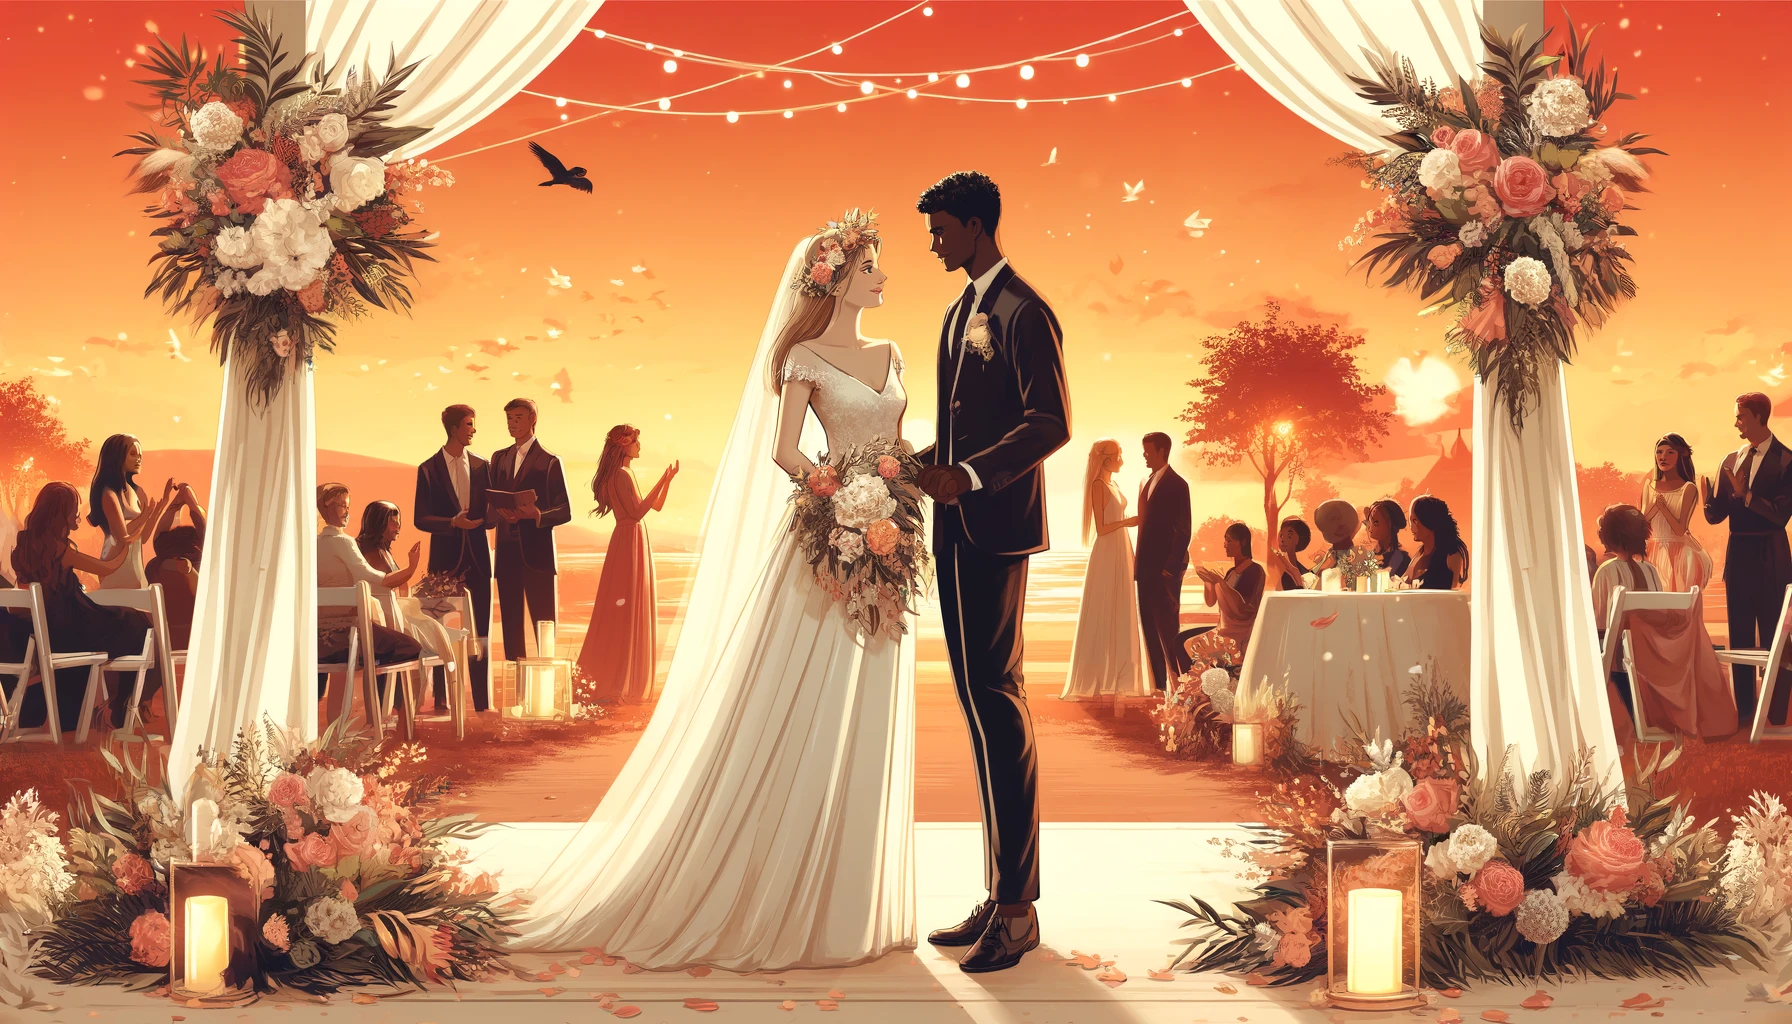
\includegraphics[width=24.89in]{images/dalle-wedding} \caption{Et blandet ægteskab, tolket af en AI model}\label{fig:fig-partner}
\end{figure}

\hypertarget{kap3}{%
\chapter{Grundskoler som mødested}\label{kap3}}

\begin{figure}
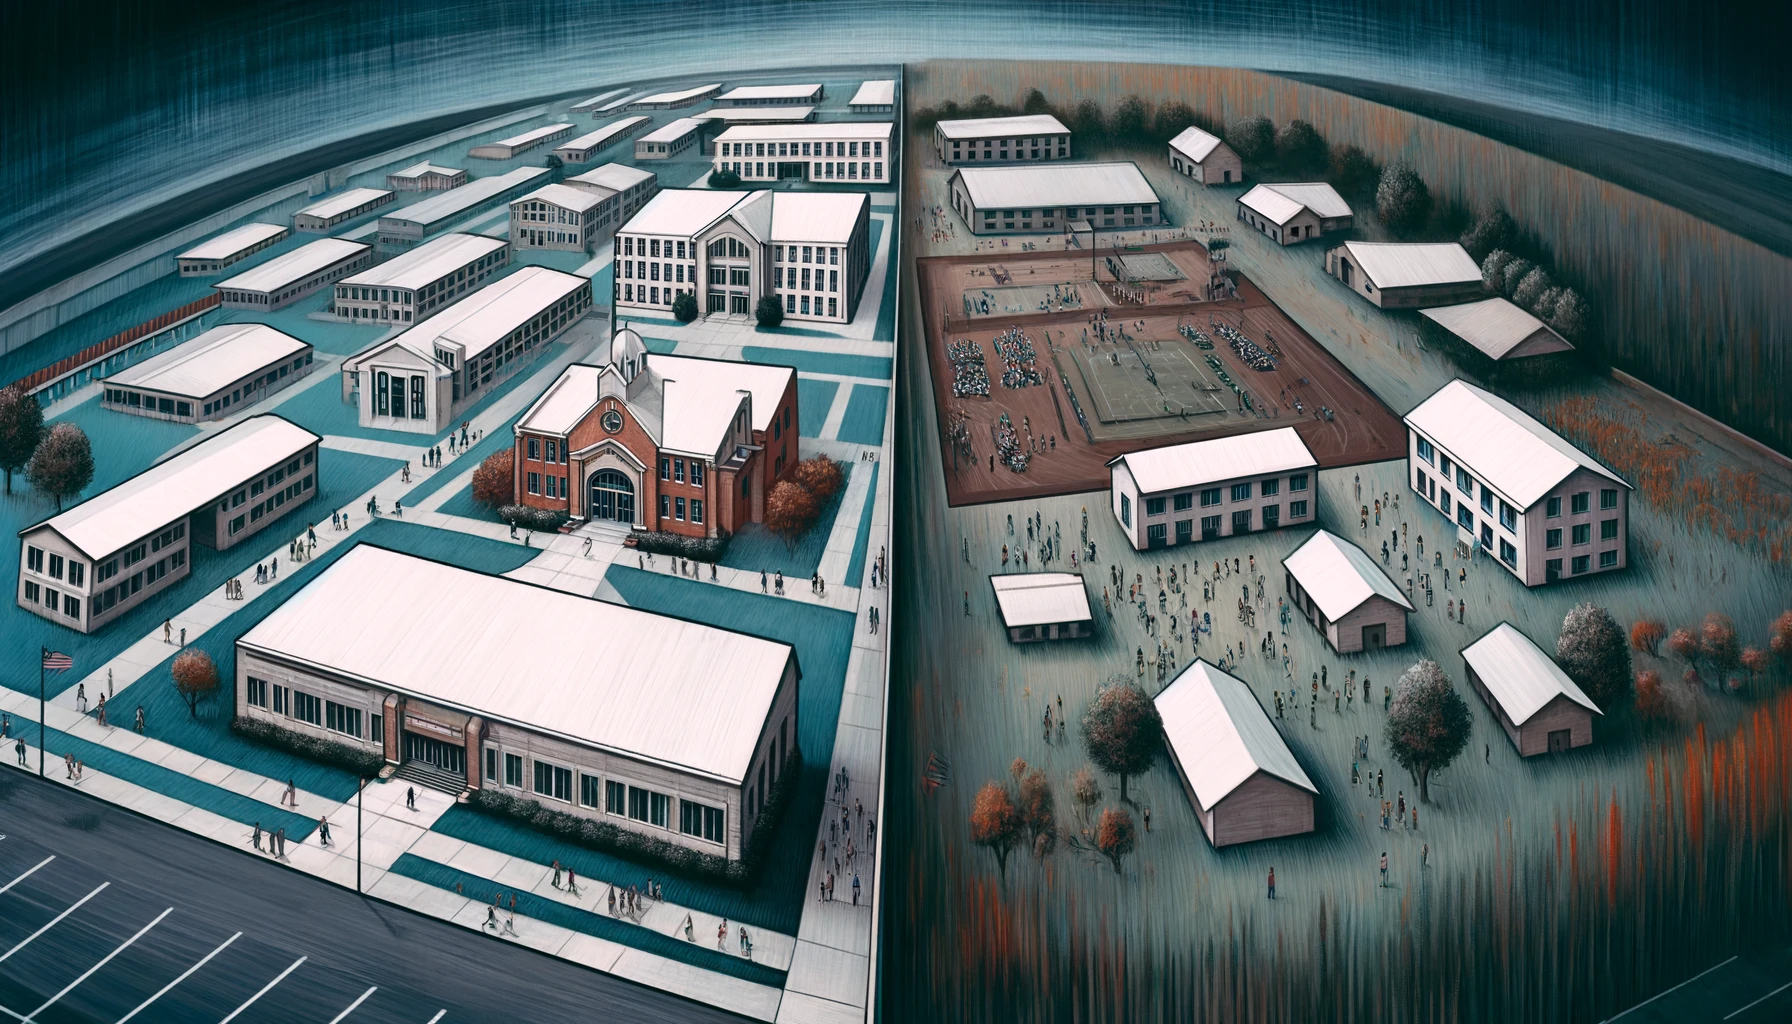
\includegraphics[width=24.89in]{images/dalle-schoolseg} \caption{Skolesegregering som det tolkes af en AI model}\label{fig:fig-schoolseg}
\end{figure}

Vi kan kryd-ref til figurer \ref{fig:fig-schoolseg}

\hypertarget{introduktion}{%
\section{Introduktion}\label{introduktion}}

Den danske grundskole er et centralt mødested mellem danskfødte, der er kendetegnet ved hvid hudfarve og kulturkristendom, og etniske minoriteter, hvoraf mange ikke deler disse kendetegn. Med andre ord, grundskolen er et rum hvor børn kan interagere med hinanden, uanset deres ligheder med andre børn og deres forældre.

Grundskolen i Danmark omfatter børn i alderen 6-16 år. Et særligt kendetegn ved den danske grundskole, sammenlignet med andre internationale skolesystemer, er fraværet af ``tracking''---elevdifferentiering--baseret på faglige evner. Det betyder, at børn ikke bliver placeret på bestemte skoler eller spor afhængigt af deres præstationer i de tidlige skoleår, som det er tilfældet i andre europæiske lande som Tyskland, Holland og England. I stedet fastlægger folkeskoleloven, at undervisningen i det danske skolesystem skal tilpasses til det pågældende klasserum gennem undervisningsdifferentiering.

I den internationale kontakt- og integrationslitteratur fremhæves skoler ofte som steder med potentiale til at nedbryde fordomme og stereotyper. Dette potentiale skyldes flere faktorer: 1) Børnene befinder sig i en kontekst, hvor der er en autoritet (læreren), der strukturerer interaktioner og opgaver. 2) Børnene forventes at have et fælles mål (læring/eksamener). 3) De arbejder sammen om dette mål i overensstemmelse med skolens didaktiske principper. 4) Børnene har samme status\footnote{Det skal selvfølgelig ikke underkendes at der er både forskning og personlige historier, der beskriver tilfælde af diskrimination og fordomme mellem lærer og minoritetselever og elever imellem (Andersen \& Guul, 2019).} i klassen (alle er elever underlagt læreren) (Allport, 1954; Pettigrew and Tropp, 2006; Tropp and Pettigrew, 2005). Optimal social kontakt i denne kontekst, som påpeget af Pettigrew (1998), er også betinget af, 5) at interaktionerne har venskabspotentiale. Da børn i en klasse har samme alder, og der som regel er en nogenlunde lige kønsfordeling i de fleste skoler, er der et principielt højt venskabspotentiale i de danske grundskoler (McPherson et al., 2001).

International forskning har vist, at børn i såkaldte ``blandede skoler'' har flere venskaber eller sociale relationer på tværs af etniske gruppeskel (Kruse and Kroneberg, 2019; Leszczensky and Pink, 2015). En anden forventet effekt er de såkaldte klassekammerateffekter (peer effect), som antager, at ressourcestærke elever kan være med til at hæve det faglige niveau for deres mindre ressourcestærke klassekammerater. Der pågår dog samtidigt diskussioner om, at både kontakt- og klassekammerateffekter i en metodologisk forstand er svære at isolere kausalt, da der forventeligt er grundlæggende problemer med selvselektion. For eksempel vil familier med de allerede laveste fordomme være mere tilbøjelige til at vælge den etnisk diverse distriktsskole (se f.eks. Hassan et al., 2022, eller Hermansen \& Birkelund, 2015 for en oversigt og diskussion).

Med det danske princip om undervisningsdifferentiering i stedet for elevdifferentiering er den danske grundskole forventeligt et eksempel på optimal realisering af positive kontakt-effekter gennem sociale relationer på tværs af grænser i et barns formative år (Larsen, 2024c; Larsen, 2016), især i betragtning af, at børnene tilbringer 10 år sammen i alle fag. Den aktuelle udfordring er imidlertid, at Danmark har en meget liberal og generøs skolevalgspolitik, hvor omkring 75\% af omkostningerne for hvert enkelt barn er statsfinansierede, mens den resterende fjerdedel er brugerbetaling, hvilket gør privatskoler tilgængelige for en stor del af befolkningen - men samtidig utilgængelige for de laveste indkomstgrupper. Dette har skabt bekymringer for, at det socialdemokratiske princip om, at børn fra forskellige baggrunde går på samme skole, ikke længere bliver realiseret, fordi forældre frit kan vælge skoler til og fra.

Historisk set går retten til at bestemme over sit barns skolegang i Danmark, under myndighedernes tilsyn, tilbage til Friskoleloven fra 1855. I dag tillader reglerne, at selvom hver adresse er tilknyttet et skoledistrikt, hvor barnet har garanteret ret til indskrivning, er familier frie til at søge en anden folke-, privat- eller friskole, enten inden for kommunen eller i en anden kommune. Det eneste lovlige grundlag, en folkeskole kan afvise et barns optagelse på, er, hvis skolen ikke har plads, hvilket defineres som 28 børn i hver klasse i den pågældende årgang\footnote{Kommuner kan dog sænke dette maksimum, for at begrænse mulighederne for anvendelsen af skolevalg. Grundet den decentrale finansiering af folkeskolen har de enkelte folkeskoler også store individuelle omkostninger ved at flytte et barn til et specialtilbud og kan i praksis ikke udelukke børn fra skolen. I modsætning har privatskolerne mindre udgifter i forbindelse med henvisninger til specialtilbud idet de søger disse midler hos staten, hvor folkeskolerne skal finde midlerne i deres kommunalt allokerede budget.}. Til forskel kan fri- og privatskoler permanent bortvise børn eller afvise optagelse baseret på en individuel vurdering, hvilket folkeskoler også kunne før 2005. Disse strukturelle forhold har affødt en grundlæggende bekymring for, at frit skolevalg og det private skolemarked vil føre til stigende ulighed og segregation mellem skoler på grund af socioøkonomiske forskelle i, hvem der i størst omfang vælger -- eller er i stand til -- at benytte sig af muligheden for frit skolevalg.

\hypertarget{kap4}{%
\chapter{Arbejdspladser som mødested}\label{kap4}}

\begin{figure}
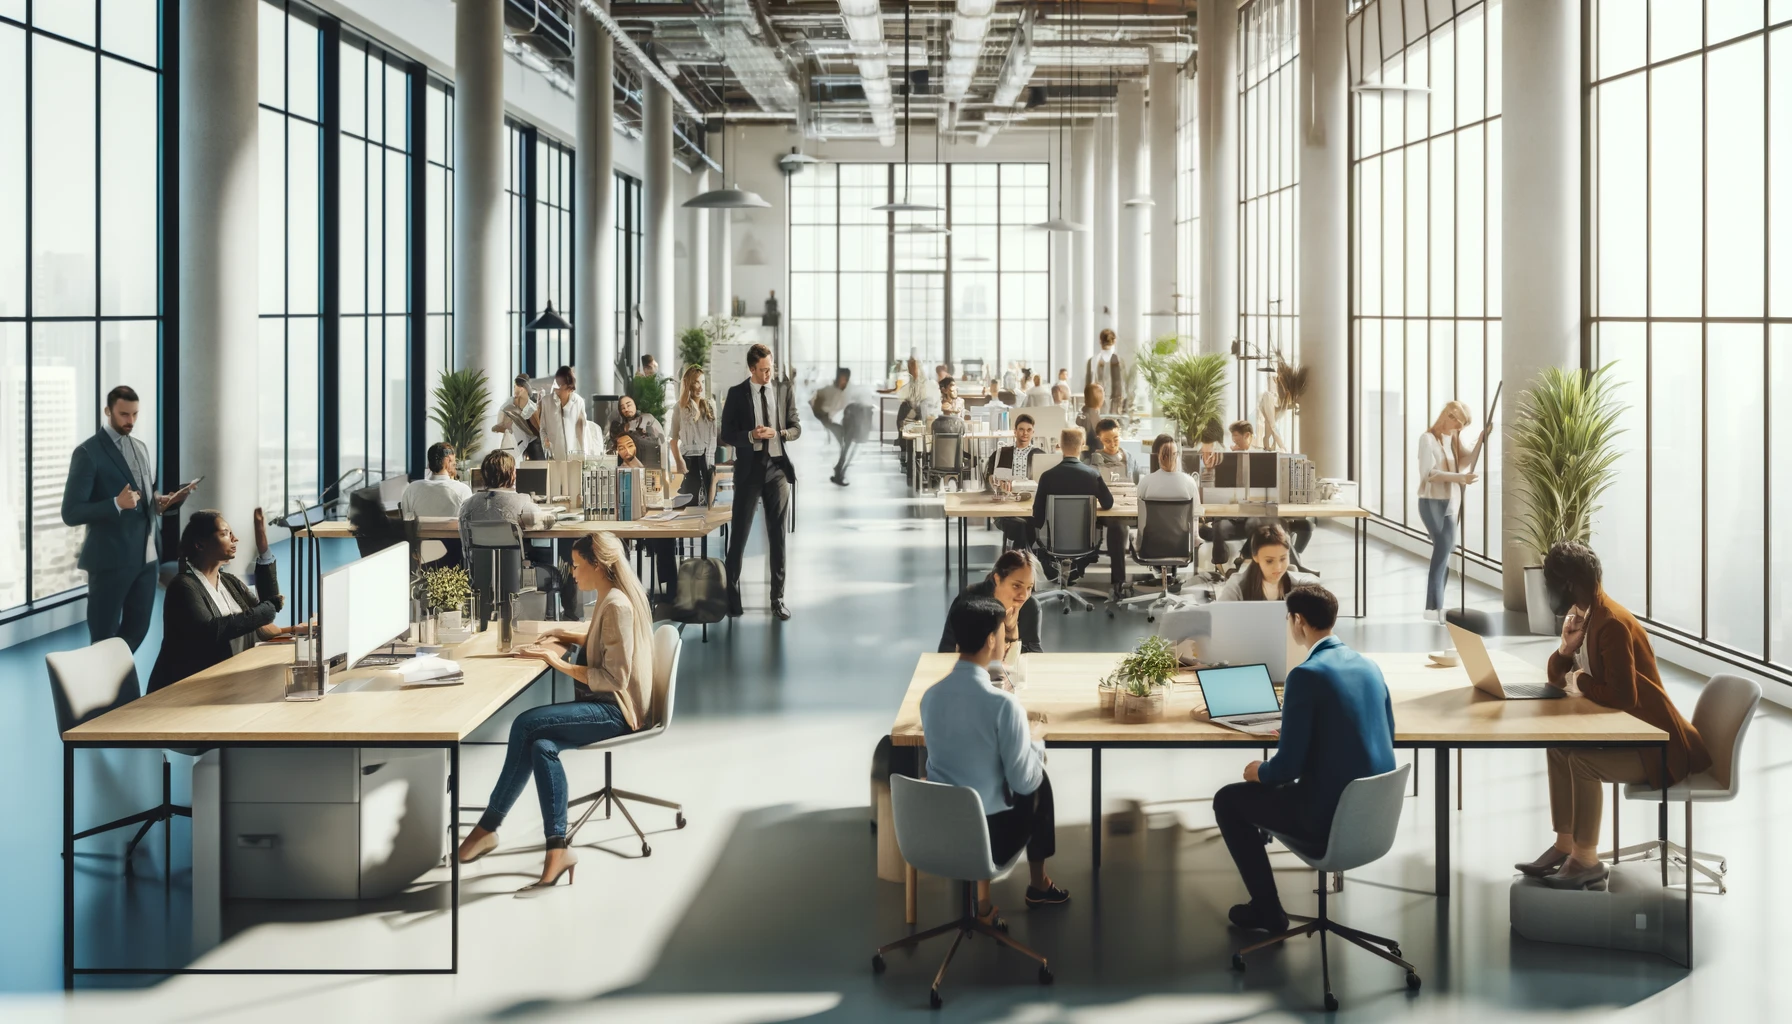
\includegraphics[width=24.89in]{images/dalle-work} \caption{En multikulturel arbejdsplads, tolket af en AI model}\label{fig:fig-work}
\end{figure}

\hypertarget{kap5}{%
\chapter{Foreninger som mødested}\label{kap5}}

\begin{figure}
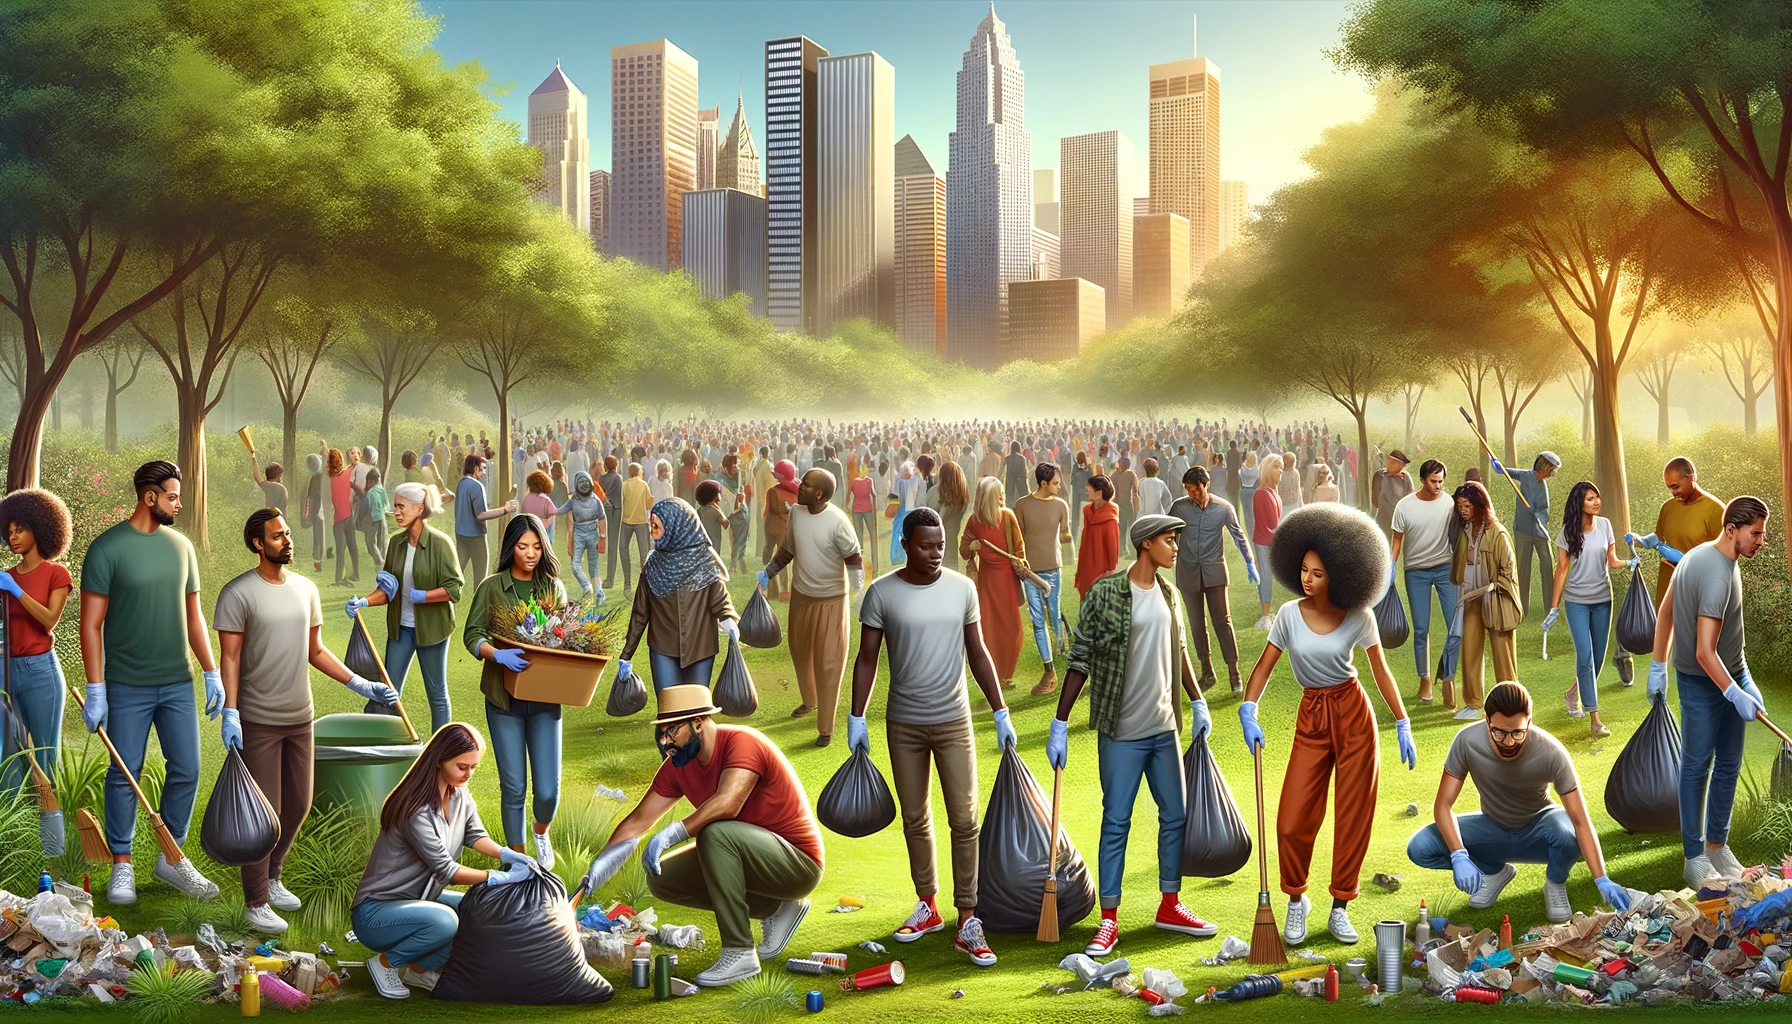
\includegraphics[width=24.89in]{images/dalle-civil} \caption{Minoriters deltagelse i civilsamfund, tolket af en AI model}\label{fig:fig-civil}
\end{figure}

\hypertarget{kap6}{%
\chapter{Venskaber -- det første skridt}\label{kap6}}

\begin{figure}
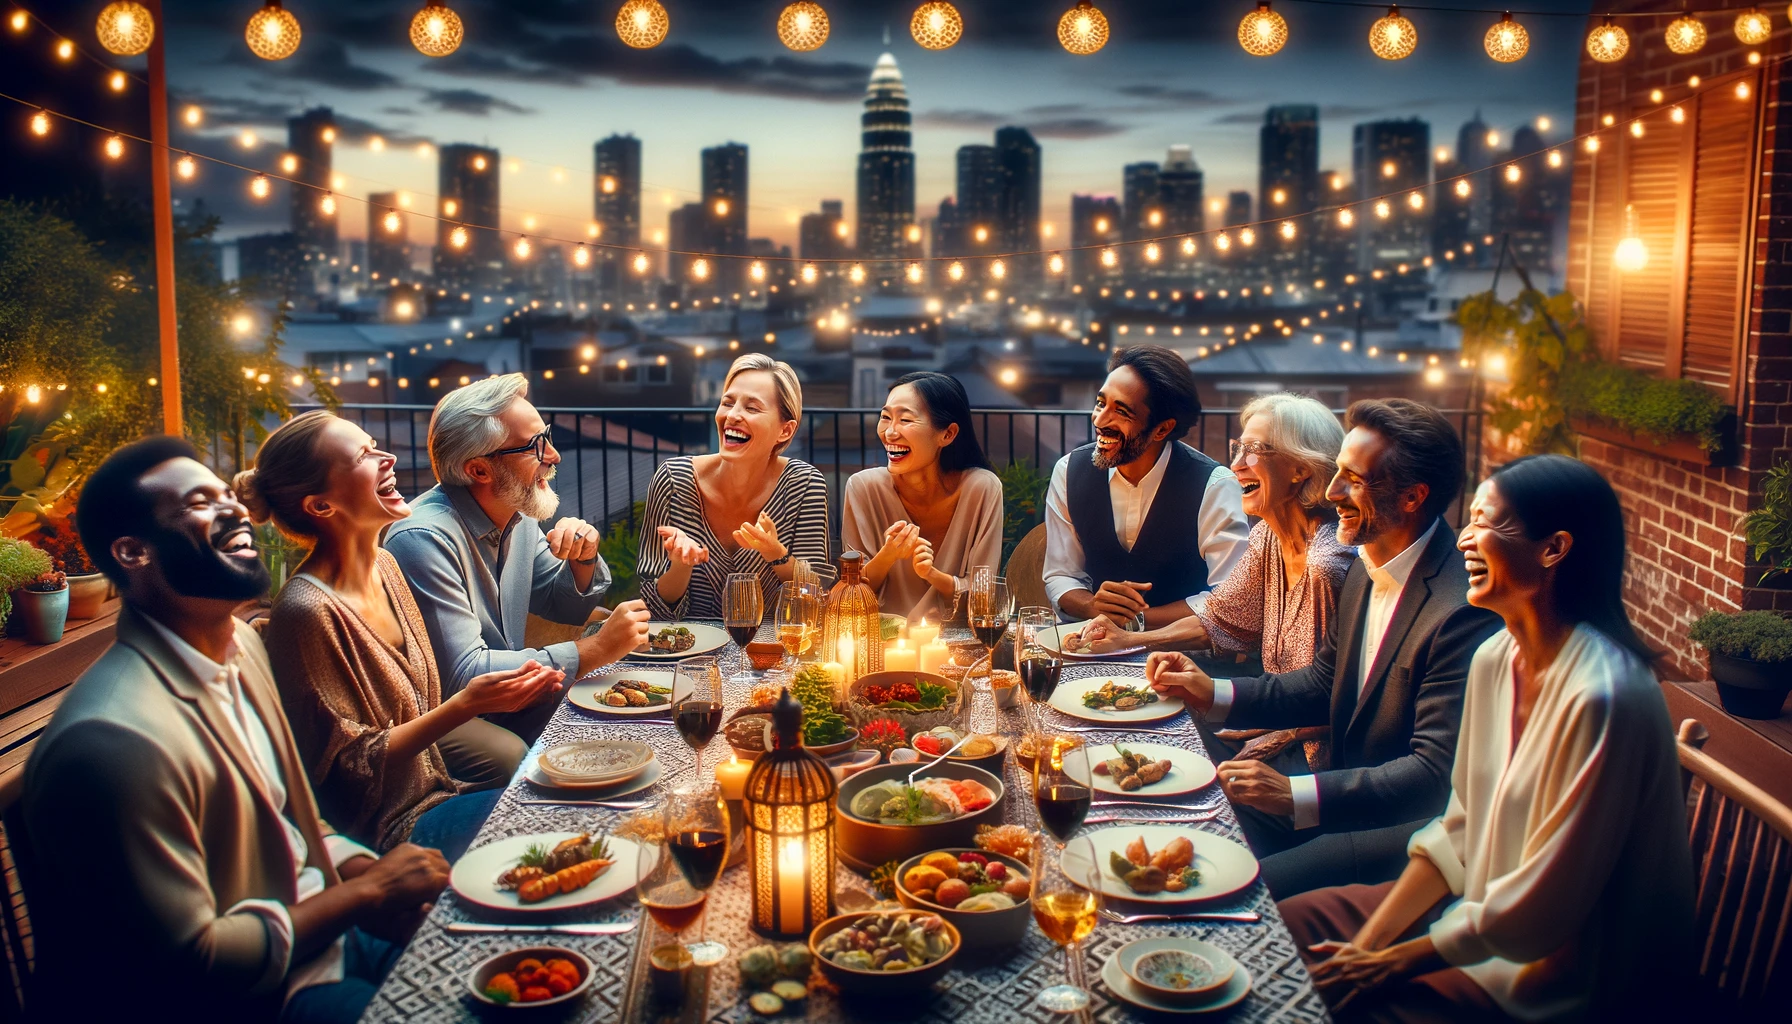
\includegraphics[width=24.89in]{images/dalle-friendships} \caption{Interetniske venskaber, tolket af en AI model}\label{fig:fig-friendships}
\end{figure}

\hypertarget{kap7}{%
\chapter{Integration i et kontaktperspektiv}\label{kap7}}

\begin{figure}
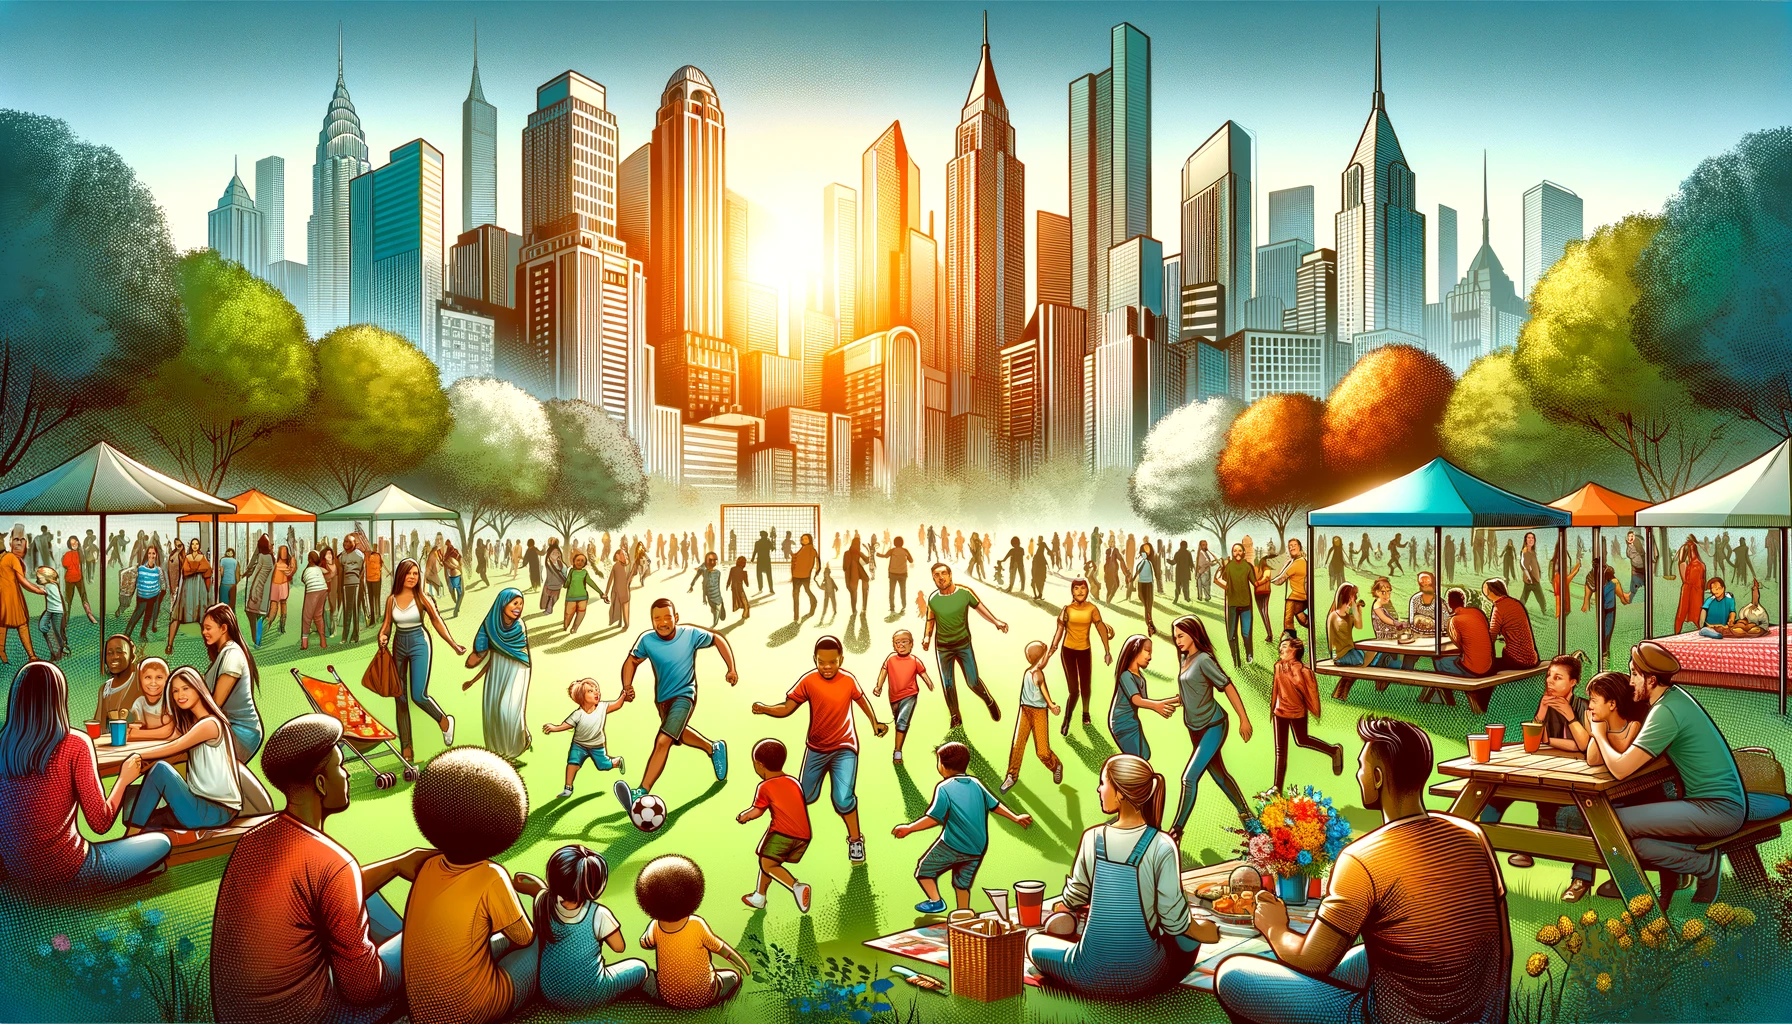
\includegraphics[width=24.89in]{images/dalle-integration} \caption{Social integration, tolket af en AI model}\label{fig:fig-integration}
\end{figure}

test \citep{xie2015}.

\hypertarget{litteraturliste}{%
\chapter*{Litteraturliste}\label{litteraturliste}}
\addcontentsline{toc}{chapter}{Litteraturliste}

\hypertarget{appendix-bilag}{%
\appendix}


\hypertarget{bilag1}{%
\chapter{Første bilag\ldots{}}\label{bilag1}}

This will be Appendix A.

\hypertarget{bilag2}{%
\chapter{Andet bilag\ldots{}}\label{bilag2}}

This will be Appendix B.

  \bibliography{book.bib,packages.bib}

\end{document}
